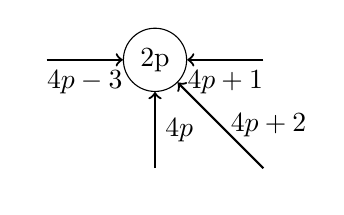
\begin{tikzpicture}[scale=0.5]

    \tikzset{nodestyle/.style={draw,shape=circle}}
    \node (p3) at ( 6, 0) {};
    \node (p4) at ( 9, 0) {};

    \node (p8) at ( 3, 3) {};
    \node[nodestyle] (p9) at ( 6, 3) {2p};
	\node (p10) at (9,3) {};

    \begin{scope}[every path/.style={->,thick}]
    	\draw (p8) -- (p9)node[midway,below]{$4p-3$}; 
        \draw (p3) -- (p9)node[midway,right]{$4p$};
        \draw (p4) -- (p9)node[midway,right]{$4p+2$};
		\draw (p10) -- (p9)node[midway,below]{$4p+1$};
    \end{scope} 
\end{tikzpicture}
